%%%%%%%%%%%%%%%%%%%%%%%%%%%%% SLIDE 4.0 %%%%%%%%%%%%%%%%%%%%%%%%%%%%%%%%%%%%%%%%%%%
\begin{frame}{{\bf \color{blue} Modelagem geométrica}}

\begin{block}{\bf Modelagem geométrica}
Conjunto de técnicas e algoritmos utilizados para modelar determinadas formas matemáticas, sujeitas a condições particulares de forma e suavidade.

\medskip

Utilizado em especial em CAD/CAM \textit{(computer aided design / manufacturing)}, por seu alto poder em modelagem de superfícies.

\medskip

Uma forma possível de se modelar é com a utilização da \destaq{discretização do operador de Laplace-Beltrami}.
\end{block}

\end{frame}

%%%%%%%%%%%%%%%%%%%%%%%%%%%%% SLIDE 4.1 %%%%%%%%%%%%%%%%%%%%%%%%%%%%%%%%%%%%%%%%%%%
\begin{frame}{{\bf \color{blue} Modelagem geométrica}}
	
	\begin{block}{\bf Métodos para modelagem}
		Com a utilização da discretização do operador de Laplace-Beltrami, existem métodos:
		\begin{itemize}
			\item baseados em malha \textit{(mesh-based)}
			\item baseados em ponto \textit{(point-based)}
		\end{itemize}
	\end{block}
\end{frame}

%%%%%%%%%%%%%%%%%%%%%%%%%%%%% SLIDE 4.1 %%%%%%%%%%%%%%%%%%%%%%%%%%%%%%%%%%%%%%%%%%%
\begin{frame}{{\bf \color{blue} Modelagem geométrica}}
	
	\begin{block}{\bf Métodos para modelagem}
		Com a utilização da discretização do operador de Laplace-Beltrami, existem métodos:
		\begin{itemize}
			\item \textbf{baseados em malha \textit{(mesh-based)}} (foco da apresentação)
			\item baseados em ponto \textit{(point-based)}
		\end{itemize}
	\end{block}
\end{frame}

\begin{frame}{{\bf \color{blue} Modelagem geométrica}}
	
	\begin{block}{\bf Malhas Poligonais}
		Uma Malha Poligonal é um conjunto de Vértices, Arestas e Faces que formam um conjunto conexo. A malha poligonal pode ser categorizada pela forma de suas faces, como malhas triangulares, quadrilaterais, ou, de fato, que utilizam qualquer polígono convexo simples. Elas também podem ser bidimensionais ou tridimensionais.
	\end{block}
	
	\begin{figure}[ht]
    \centering
        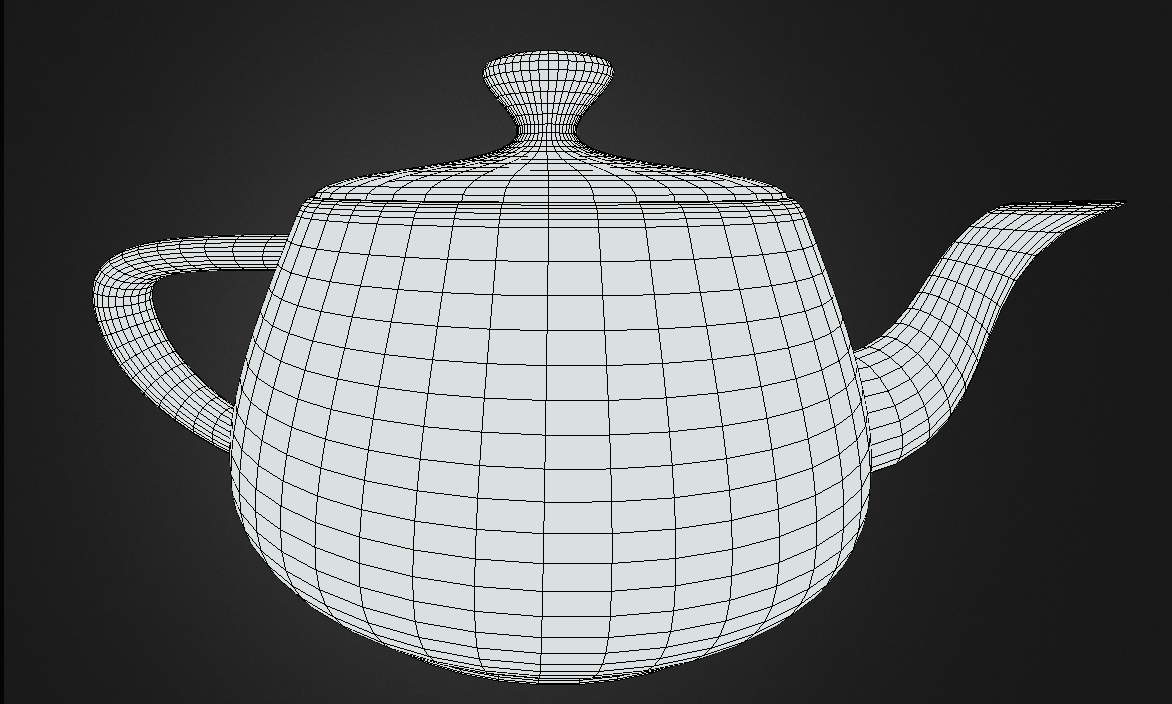
\includegraphics[width=0.5\linewidth]{imagens/Utah Teapot.PNG}
        \caption{Malha Quadrilateral Tridimensional do Bule de Utah
        \cite{utahteapot}}
        \label{fig:my_label}
    \end{figure}
\end{frame}